\documentclass[a4paper,12pt]{article}

\usepackage[utf8]{inputenc}
\usepackage{lmodern}
\usepackage[margin=1cm]{geometry}
\usepackage{amsmath}
\usepackage{graphicx}
\usepackage{xcolor}
\usepackage{caption}
\usepackage{tikz}
\usetikzlibrary{arrows.meta,positioning,shapes.geometric,calc,fit}

\pagestyle{empty}

\begin{document}
\begin{figure}[p]
  \centering
  \resizebox{\textwidth}{!}{%
  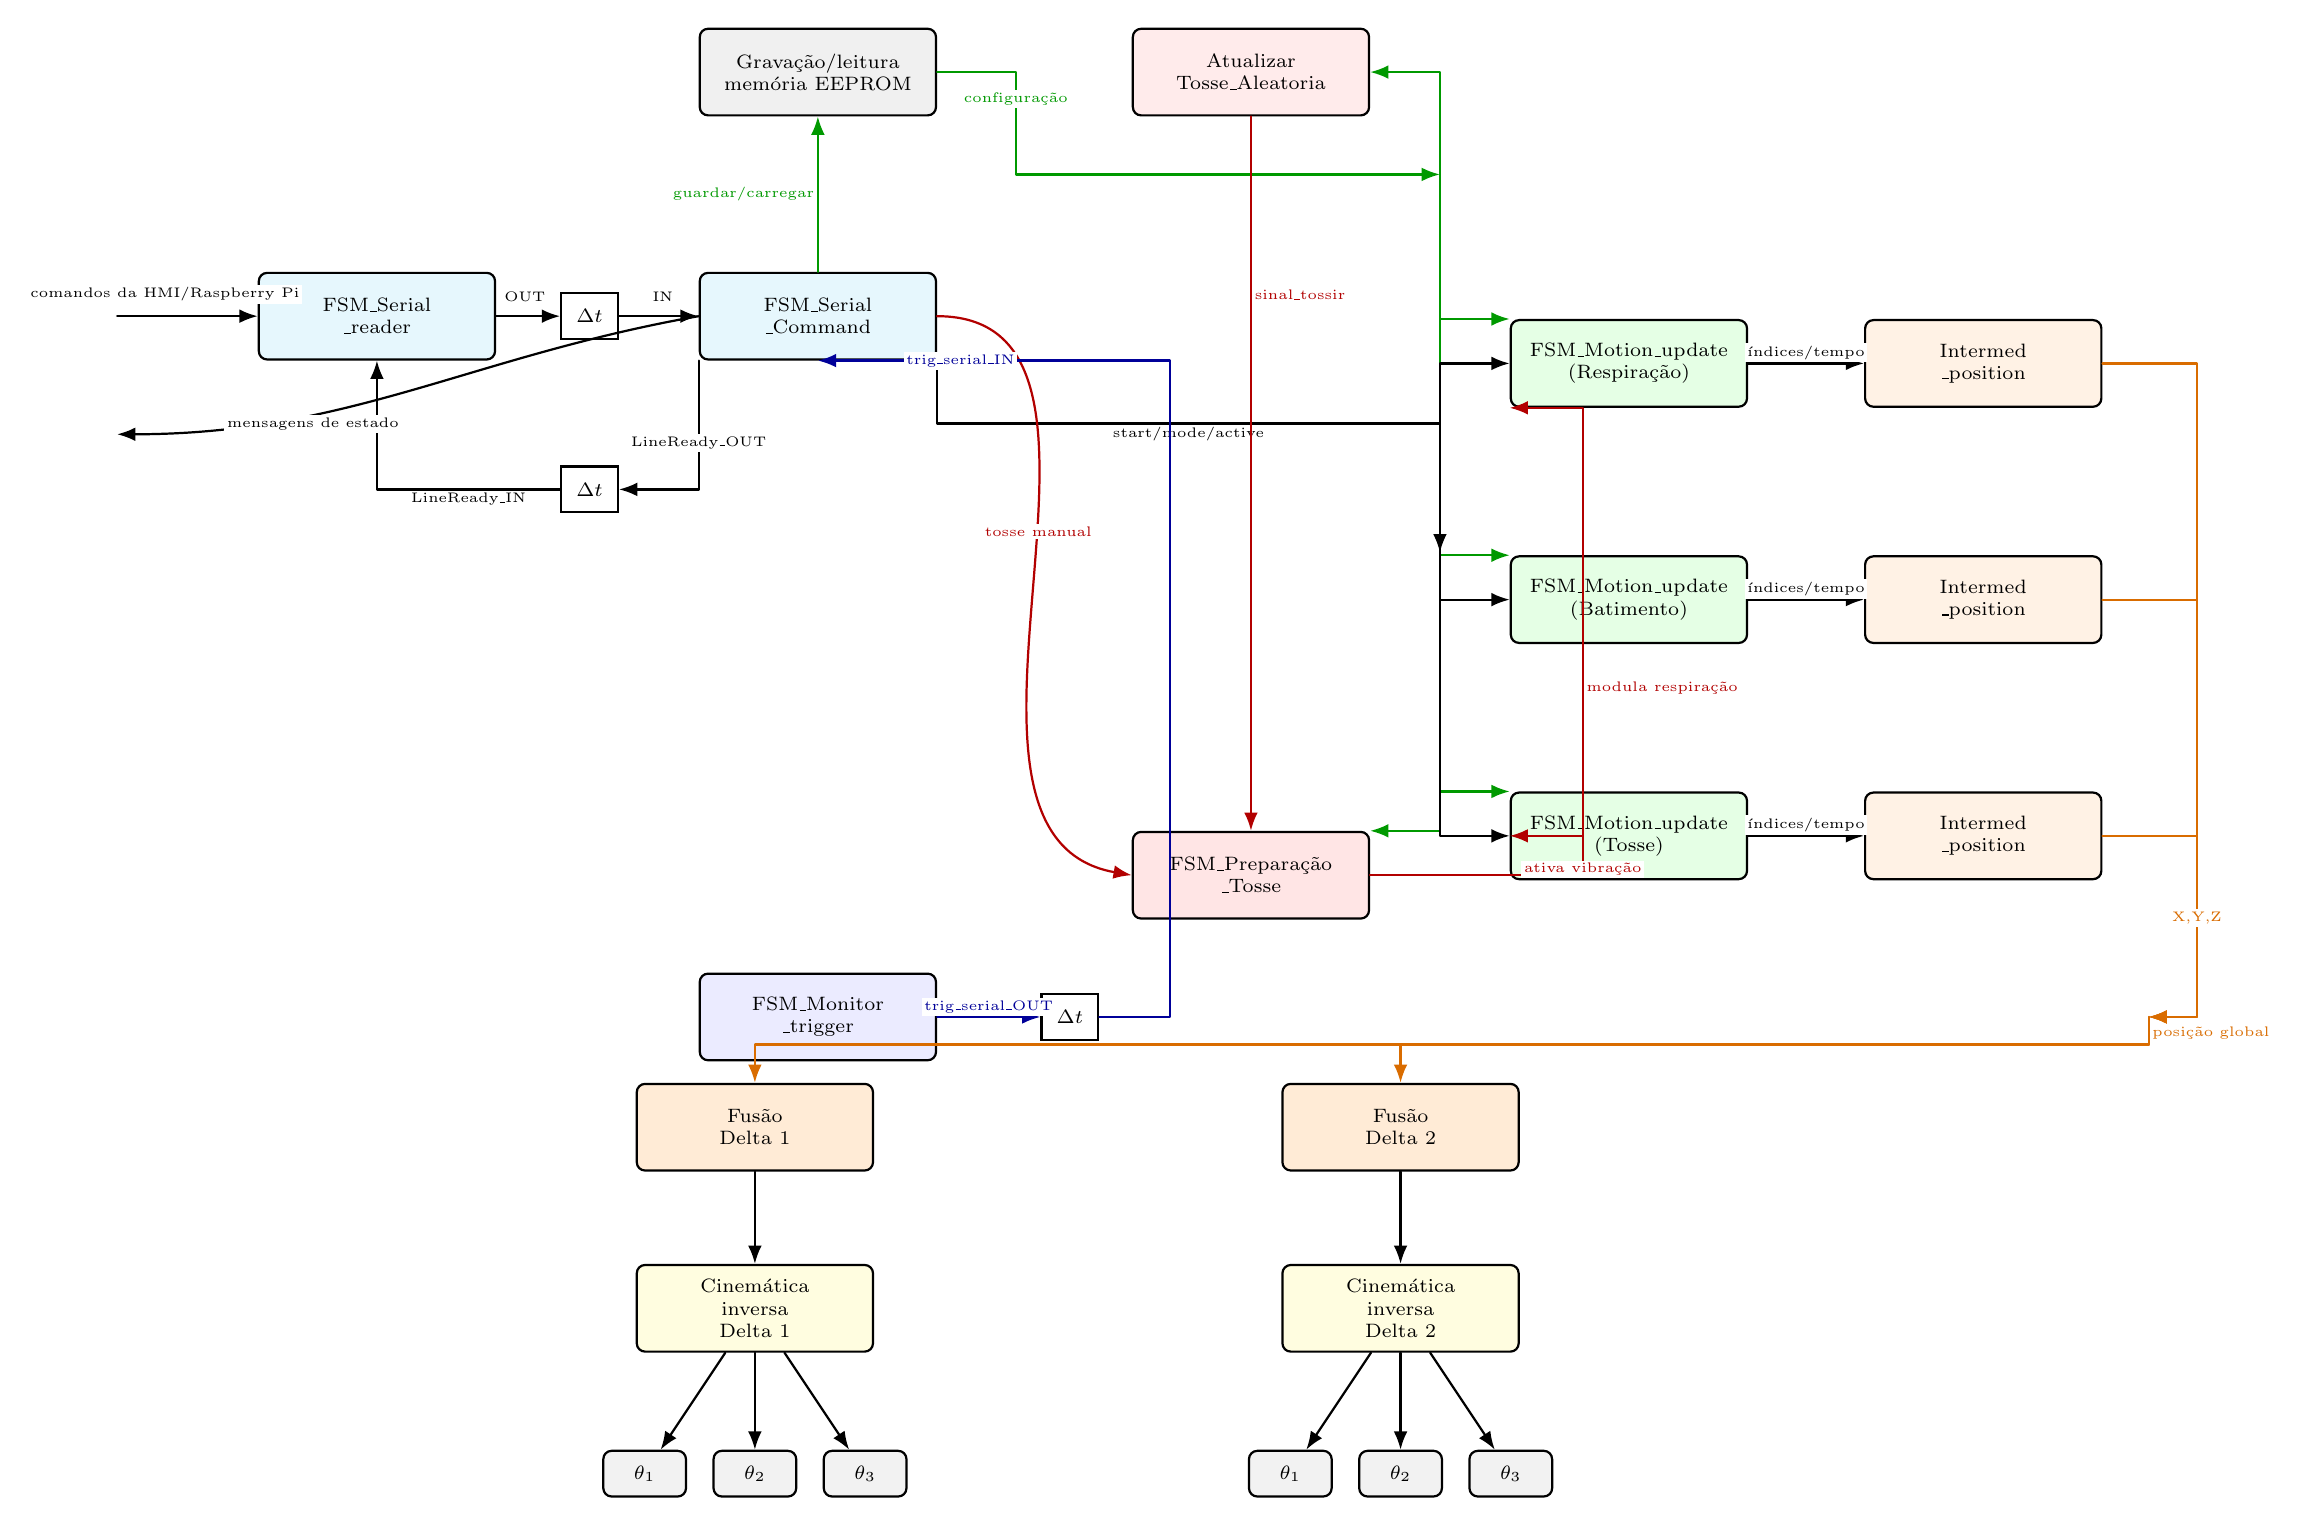
\begin{tikzpicture}[
    xscale=1.0, yscale=1.0,
    block/.style={draw, rounded corners=3pt, align=center, minimum width=3.0cm, minimum height=1.1cm, thick, font=\scriptsize},
    small/.style={draw, rounded corners=3pt, align=center, minimum width=1.05cm, minimum height=0.58cm, thick, font=\scriptsize},
    delay/.style={draw, align=center, minimum width=0.72cm, minimum height=0.58cm, thick, font=\scriptsize, fill=white},
    arrow/.style={-Latex, thick, line cap=round, line join=round},
    cfg/.style={-Latex, thick, green!60!black, line cap=round, line join=round},
    event/.style={-Latex, thick, red!70!black, line cap=round, line join=round},
    positionflow/.style={-Latex, thick, orange!85!black, line cap=round, line join=round},
    timeflow/.style={-Latex, thick, blue!60!black, line cap=round, line join=round},
    lab/.style={font=\tiny, fill=white, inner sep=1pt}
  ]
    \node[block, fill=cyan!10]  (reader) at (-8.0,14.0) {FSM\_Serial\\\_reader};
    \node[delay] (dtSerial) at (-5.3,14.0) {\(\Delta t\)};
    \node[block, fill=cyan!10]  (interp) at (-2.4,14.0) {FSM\_Serial\\\_Command};
    \node[delay] (dtReader) at (-5.3,11.8) {\(\Delta t\)};
    \node[block, fill=gray!12]  (eeprom) at (-2.4,17.1) {Gravação/leitura\\memória EEPROM};

    \node[block, fill=blue!8]   (monitor) at (-2.4,5.1) {FSM\_Monitor\\\_trigger};
    \node[delay] (dtMonitor) at (0.8,5.1) {\(\Delta t\)};

    \node[block, fill=red!8]   (ttrig) at (3.1,17.1) {Atualizar\\Tosse\_Aleatoria};
    \node[block, fill=red!10]  (tprep) at (3.1,6.9) {FSM\_Preparação\\\_Tosse};

    \node[block, fill=green!10] (mresp)  at (7.9,13.4) {FSM\_Motion\_update\\(Respiração)};
    \node[block, fill=green!10] (mbat)   at (7.9,10.4) {FSM\_Motion\_update\\(Batimento)};
    \node[block, fill=green!10] (mtosse) at (7.9,7.4)  {FSM\_Motion\_update\\(Tosse)};

    \node[block, fill=orange!10] (ipresp)  at (12.4,13.4) {Intermed\\\_position};
    \node[block, fill=orange!10] (ipbat)   at (12.4,10.4) {Intermed\\\_position};
    \node[block, fill=orange!10] (iptosse) at (12.4,7.4)  {Intermed\\\_position};

    \node[block, fill=orange!16] (fus1) at (-3.2,3.7) {Fusão\\Delta 1};
    \node[block, fill=orange!16] (fus2) at (5.0,3.7)  {Fusão\\Delta 2};
    \node[block, fill=yellow!12] (ik1) at (-3.2,1.4) {Cinemática\\inversa\\Delta 1};
    \node[block, fill=yellow!12] (ik2) at (5.0,1.4) {Cinemática\\inversa\\Delta 2};

    \node[small, fill=gray!10] (s11) at (-4.6,-0.7) {\(\theta_1\)};
    \node[small, fill=gray!10] (s12) at (-3.2,-0.7) {\(\theta_2\)};
    \node[small, fill=gray!10] (s13) at (-1.8,-0.7) {\(\theta_3\)};
    \node[small, fill=gray!10] (s21) at (3.6,-0.7)  {\(\theta_1\)};
    \node[small, fill=gray!10] (s22) at (5.0,-0.7)  {\(\theta_2\)};
    \node[small, fill=gray!10] (s23) at (6.4,-0.7)  {\(\theta_3\)};

    \coordinate (cfgBus) at (5.5,15.8);
    \coordinate (motionBus) at (5.5,11.0);
    \coordinate (posBus) at (14.5,5.1);

    \draw[arrow] (-11.3,14.0) -- node[lab, pos=0.34, above, yshift=4pt]{comandos da HMI/Raspberry Pi} (reader.west);
    \draw[arrow] (reader.east) -- node[lab, pos=0.45, above, yshift=4pt]{OUT} (dtSerial.west);
    \draw[arrow] (dtSerial.east) -- node[lab, pos=0.55, above, yshift=4pt]{IN} (interp.west);
    \draw[arrow] (interp.south west) |- node[lab, pos=0.28, below]{LineReady\_OUT} (dtReader.east);
    \draw[arrow] (dtReader.west) -| node[lab, pos=0.25, below]{LineReady\_IN} (reader.south);
    \draw[arrow] (interp.west) to[out=190,in=0] node[lab, pos=0.68, below]{mensagens de estado} (-11.3,12.5);

    \draw[cfg] (interp.north) -- node[lab, left]{guardar/carregar} (eeprom.south);
    \draw[cfg] (eeprom.east) -- ++(1.0,0) |- node[lab, pos=0.18, above]{configuração} (cfgBus);
    \draw[cfg] (cfgBus) |- (mresp.north west);
    \draw[cfg] (cfgBus) |- (mbat.north west);
    \draw[cfg] (cfgBus) |- (mtosse.north west);
    \draw[cfg] (cfgBus) |- (tprep.north east);
    \draw[cfg] (cfgBus) |- (ttrig.east);

    \draw[arrow] (interp.south east) -- ++(0,-0.8) -| node[lab, pos=0.25, below]{start/mode/active} (motionBus);
    \draw[arrow] (motionBus) |- (mresp.west);
    \draw[arrow] (motionBus) |- (mbat.west);
    \draw[arrow] (motionBus) |- (mtosse.west);

    \draw[event] (ttrig.south) -- node[lab, pos=0.25, right]{sinal\_tossir} (tprep.north);
    \draw[event] (interp.east) to[out=0,in=170] node[lab, pos=0.45, above]{tosse manual} (tprep.west);
    \draw[event] (tprep.east) -- ++(2.7,0) |- node[lab, pos=0.2, right]{modula respiração} (mresp.south west);
    \draw[event] (tprep.east) -- ++(2.7,0) |- node[lab, pos=0.2, below]{ativa vibração} (mtosse.west);

    \draw[timeflow] (monitor.east) -- node[lab, above]{trig\_serial\_OUT} (dtMonitor.west);
    \draw[timeflow] (dtMonitor.east) -- ++(0.9,0) |- node[lab, pos=0.88, right]{trig\_serial\_IN} (interp.south);

    \draw[arrow] (mresp.east) -- node[lab, above]{índices/tempo} (ipresp.west);
    \draw[arrow] (mbat.east) -- node[lab, above]{índices/tempo} (ipbat.west);
    \draw[arrow] (mtosse.east) -- node[lab, above]{índices/tempo} (iptosse.west);

    \draw[positionflow] (ipresp.east) -- ++(1.2,0) |- (posBus);
    \draw[positionflow] (ipbat.east) -- ++(1.2,0) |- (posBus);
    \draw[positionflow] (iptosse.east) -- ++(1.2,0) |- node[lab, pos=0.2, below]{X,Y,Z} (posBus);
    \draw[positionflow] (posBus) -- node[lab, pos=0.58, right]{posição global} ++(0,-0.35) -| (fus1.north);
    \draw[positionflow] (posBus) -- ++(0,-0.35) -| (fus2.north);

    \draw[arrow] (fus1) -- (ik1);
    \draw[arrow] (fus2) -- (ik2);
    \draw[arrow] (ik1) -- (s11);
    \draw[arrow] (ik1) -- (s12);
    \draw[arrow] (ik1) -- (s13);
    \draw[arrow] (ik2) -- (s21);
    \draw[arrow] (ik2) -- (s22);
    \draw[arrow] (ik2) -- (s23);
  \end{tikzpicture}}
  \caption{Estrutura global das máquinas de estados e blocos de controlo do firmware, com os atrasos de um ciclo representados por \(\Delta t\).}
  \label{fig:arquitetura-software}
\end{figure}

\end{document}
